% Created 2017-03-13 Mon 10:44
% Intended LaTeX compiler: pdflatex
\documentclass[11pt]{article}
\usepackage[utf8]{inputenc}
\usepackage[T1]{fontenc}
\usepackage{graphicx}
\usepackage{grffile}
\usepackage{longtable}
\usepackage{wrapfig}
\usepackage{rotating}
\usepackage[normalem]{ulem}
\usepackage{amsmath}
\usepackage{textcomp}
\usepackage{amssymb}
\usepackage{capt-of}
\usepackage{hyperref}
\date{\today}
\title{CS-322: Introduction to Database Systems}
\hypersetup{
 pdfauthor={},
 pdftitle={CS-322: Introduction to Database Systems},
 pdfkeywords={},
 pdfsubject={},
 pdfcreator={Emacs 25.1.1 (Org mode 9.0.5)}, 
 pdflang={English}}
\begin{document}

\maketitle
\setcounter{tocdepth}{2}
\tableofcontents

\section{Administrative stuff}
\label{sec:org9d6bd25}
\subsection{Reading}
\label{sec:org86ddf94}
\begin{itemize}
\item \href{Ramakrishnan\%20-\%20Database\%20Management\%20Systems\%203rd\%20Edition.pdf}{Book}
\item Papers
\end{itemize}
\subsection{Grading}
\label{sec:org3525cb0}
\begin{itemize}
\item Midterm 30\%
\item Project 30\%
\item Final   40\% (During summer exam session)
\end{itemize}
\section{Lecture 1}
\label{sec:org0a91a8e}
\subsection{Data vs Infororg-caldavmation}
\label{sec:org6329b3b}
Data:
\begin{itemize}
\item Facts
\end{itemize}
org-caldav- Basis for reasoning,\ldots{}
\begin{itemize}
\item Can be useful/reorg-caldavlevant or not
\item Must be processed
\end{itemize}
When organized/processed, becomes Information:
\begin{itemize}
\item Meaningful
\item Relevant
\item \textbf{Actionable} leads to a solution
\end{itemize}
\subsection{Look up house of cards big data \href{http://wwInternet analyticsw.bigwisdom.net/blog/2016/03/13/4-big-data-lessons-from-house-of-cards/}{here}}
\label{sec:orgfed6146}
\subsection{Look up \href{https://www.emc.com/collateral/analyst-reports/idc-the-digital-universe-in-2020.pdf}{emc report for 2020}}
\label{sec:org2bf3aa6}
\subsection{Database Management System (DBMS)}
\label{sec:orgde62b83}
\begin{itemize}
\item DBMS is a software to \textbf{store}, \textbf{manager} and \textbf{facilitate access} to databases.
\item DBMS = Interrelated data (database) + set of program + se;; refile setup
;;

;; targets include this file and any file contributing to the agenda, up to 9 levels deep
(setq org-refile-targets (quote ((nil :maxlevel . 9)
\end{itemize}
(org-agenda-files :maxlevel . 9))))t of p(with-eval-after-load 'orgrograms to
  access it (software).
\begin{itemize}
\item DBMS provides \textbf{efficient} (thousands of queries/update per second), \textbf{reliable}
(availability), \textbf{convenient} (physical data indep, high level query languages)
and \textbf{safe} (protect data from failures: h/w,s/w,power, malicious users)
\textbf{multi-user} (concu(cfw:open-org-calendar)rrency) storage of and access to \textbf{massive} (extremly large
TB everyday) amounts of \textbf{persistent} (data outlives programs that operate on
it) data.
\end{itemize}
\subsection{Database}
\label{sec:org22cb52f}
\begin{itemize}
\item A \textbf{large}, \textbf{integrated}, \textbf{structured collection} of data.
\item Usually intended to model some real-world enterprise.
\item Entities and Relationships.
\end{itemize}
\subsubsection{Is WWW a DBMS?}
\label{sec:org6f52a92}
\begin{itemize}
\item Sophisticated search available
\item But not really DBMS, data unstructured, "correct answer" not well defined, few
guarantees.
\end{itemize}
\subsubsection{Is FS a DBMS?}
\label{sec:org1e6c8e3}
No, no guarantees when conflict (two edit at same time) or when power out\ldots{}
\subsection{DBMS Design and Architecture}
\label{sec:orgd0e6048}
\subsubsection{Describing Data}
\label{sec:org1d0702e}
\begin{itemize}
\item \textbf{Data model} is a collection of concepts for describing data
\item \textbf{Relation data model}, relation (table with row and columns), schema
(structure (columns) of a relation)
\item \textbf{Nested data model}, not all data fits naturally in tables
\item \textbf{Schema vs. Data}, type vs variable
\end{itemize}
\subsubsection{Logical and physical data independence}
\label{sec:org51f5da5}
\begin{itemize}
\item \textbf{Data independence} is the ability to change the
\end{itemize}
schema at one level of the database system without
changing the schema at the next higher level
\begin{itemize}
\item \textbf{Logical data independence} is the capacity to change
\end{itemize}
the conceptual schema without changing the user
views
\begin{itemize}
\item \textbf{Physical data independence} is the capacity to
\end{itemize}
change the internal schema without having to
change the conceptual schema or user views
\(\Rightarrow\) allows for modularity
\section{Lecture 2}
\label{sec:org5bf52d6}
\subsection{Data model}
\label{sec:org61f1c6b}
\begin{itemize}
\item A \textbf{data model} is a collection of concepts for describing data
\begin{itemize}
\item High-level : hides lot of low-level storage details
\item Relational, XML, Graph, Object-Oriented,\ldots{}
\end{itemize}
\item \textbf{Relational data model}
\begin{itemize}
\item Set of records
\item \textbf{Relation}: Table with rows and columns
\item \textbf{Schema}: Describes the structure (columns) of a relation
\end{itemize}
\item \textbf{Schema vs. Data}
\begin{itemize}
\item Type vs. variable
\item Description of a particular collection of data, using a given data model
\end{itemize}
\end{itemize}
\subsection{Conceptual design}
\label{sec:orgb65d460}
\begin{itemize}
\item What are the \textbf{entities} and \textbf{relationships}?
\item What info should be stored?
\item What are the \textbf{integrity constraints}?
\end{itemize}
\subsection{Entity-Relationships Model Basics}
\label{sec:org2b2ca32}
\subsubsection{Entity}
\label{sec:org239b8d2}
\begin{itemize}
\item Real-world object distinguishable from other objects.
\item An entity is described (in DB) using a set of attributes
\end{itemize}
\subsubsection{Entity Set}
\label{sec:org796867f}
\begin{itemize}
\item A collection of similar entities. E.g., all employees
\item All entities in an entity set have the same set of attributes. (Until we
consider hierarchies, anyway!)
\item Each entity set has a \textbf{key} (underlined)
\item Each attribute has a \textbf{domain}
\end{itemize}
\subsubsection{Relationship}
\label{sec:orgc6acdbf}
\begin{itemize}
\item Association among two or more entities. E.g., Fred works in Pharmacy
\end{itemize}
department
\begin{itemize}
\item Can have their own attributes
\end{itemize}
\subsubsection{Relationship Set}
\label{sec:org4251109}
A collection of similar relationships. E.g., all employees
\subsection{Constraints}
\label{sec:org4d248fa}
Limits the freedom of the data
\subsubsection{Key Constraints}
\label{sec:org289e67c}
\begin{itemize}
\item An employee can work in many departments; a department can have many
employees: \textbf{Many-to-Many}
\item In contrast, each department has at most one manager, according to the key
constraint on Manages: \textbf{One-to-Many}
\item Each driver can drive at most one vehicle and each vehicle will have at most
one driver: \textbf{One-to-One}
\end{itemize}
/!$\backslash$ \textbf{At most}, i.e. >= 1
\subsubsection{Participation Constraints}
\label{sec:orgebca9ad}
\begin{itemize}
\item Every Employee should work in at least one department
\item Every Department should have at least one employee
\end{itemize}
\(\Rightarrow\) \textbf{Total participation}

\begin{itemize}
\item There could be some Employees who are not managers
\item Every Department should have at least one manager
\end{itemize}
If also at most, then it means: "\textbf{exactly one}"

\begin{itemize}
\item There could be some Customers who do not buy any Products
\item There could be some Products which are not bought by any Customer
\end{itemize}
\(\Rightarrow\) \textbf{Partial Participation}

\begin{center}
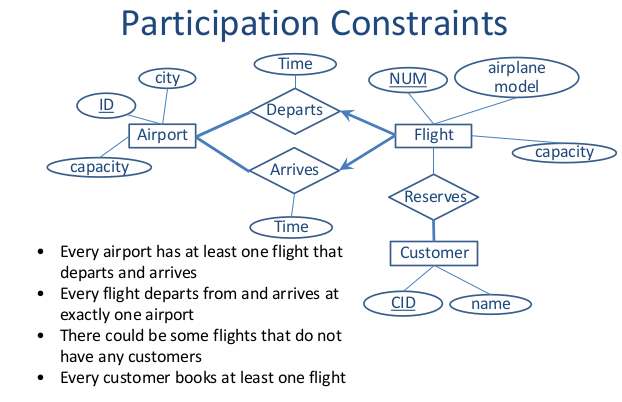
\includegraphics[width=.9\linewidth]{/home/raph/org/school/2016-2017/secondSemester/files/db_participation_constraints.png}
\end{center}
\subsubsection{Weak Entities}
\label{sec:orgd84bcd2}
A weak entity can be identified uniquely only by considering the primary key of
another (owner) entity
\begin{itemize}
\item Owner entity set and weak entity set must participate in a one-to-many
relationship set (one owner, many weak entities)
\item Weak entity set must have total participation in this identifying relationship
set
\end{itemize}
Weak entities have only a “partial key” (dashed underline)
\begin{center}
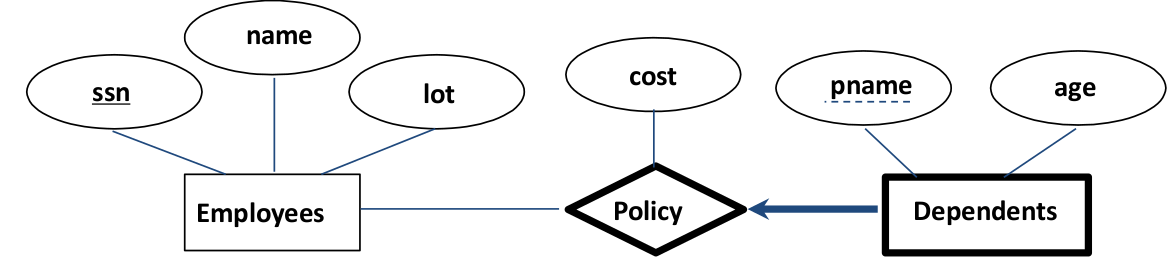
\includegraphics[width=.9\linewidth]{/home/raph/org/school/2016-2017/secondSemester/files/database_weak_entities.png}
\end{center}
\subsubsection{Ternary Relationships}
\label{sec:org2437617}
\begin{center}
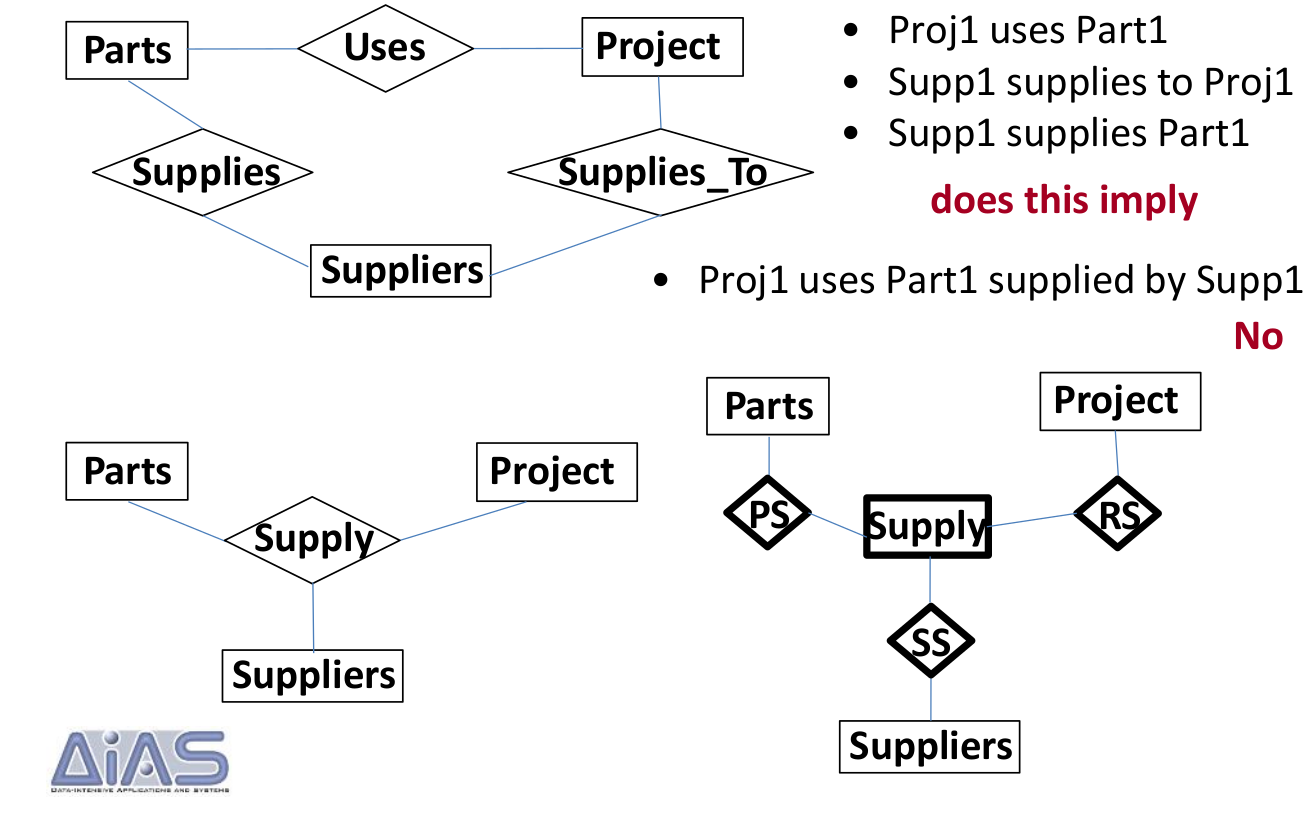
\includegraphics[width=.9\linewidth]{/home/raph/org/school/2016-2017/secondSemester/files/database_ternary.png}
\end{center}
\begin{itemize}
\item Proj1 uses Part1
\item Supp1 supplies to Proj1
\item Supp1 supplies Part1
\end{itemize}
does this imply
\begin{itemize}
\item Proj1 uses Part1 supplied by Supp1
\end{itemize}
\(\Rightarrow\) No

Can be done for n-ary relationships
\subsection{Complex relationships}
\label{sec:org92d43d7}
\subsubsection{ISA ('is a') Hierarchies}
\label{sec:org75aa39e}
\begin{itemize}
\item As in C++, or other PLs, attributes are inherited.
\item If we declare A ISA B, every A entity is also considered to be a B entity.

\item \textbf{Overlap constraints}: Can Joe be an HourlyEmps as well as a ContractEmps
entity? (Allowed/Disallowed)
\item \textbf{Covering constraints}: Does every Employees entity also have to be an
HourlyEmps or a ContractEmps entity? (Yes/No)
\item Reasons for using ISA:
\begin{itemize}
\item To add descriptive attributes specific to a subclass. (i.e., not appropriate
for all entities in the superclass)
\item To identify entities that participate in a particular relationship (i.e., not
all superclass entities participate)
\end{itemize}
\end{itemize}
\begin{center}
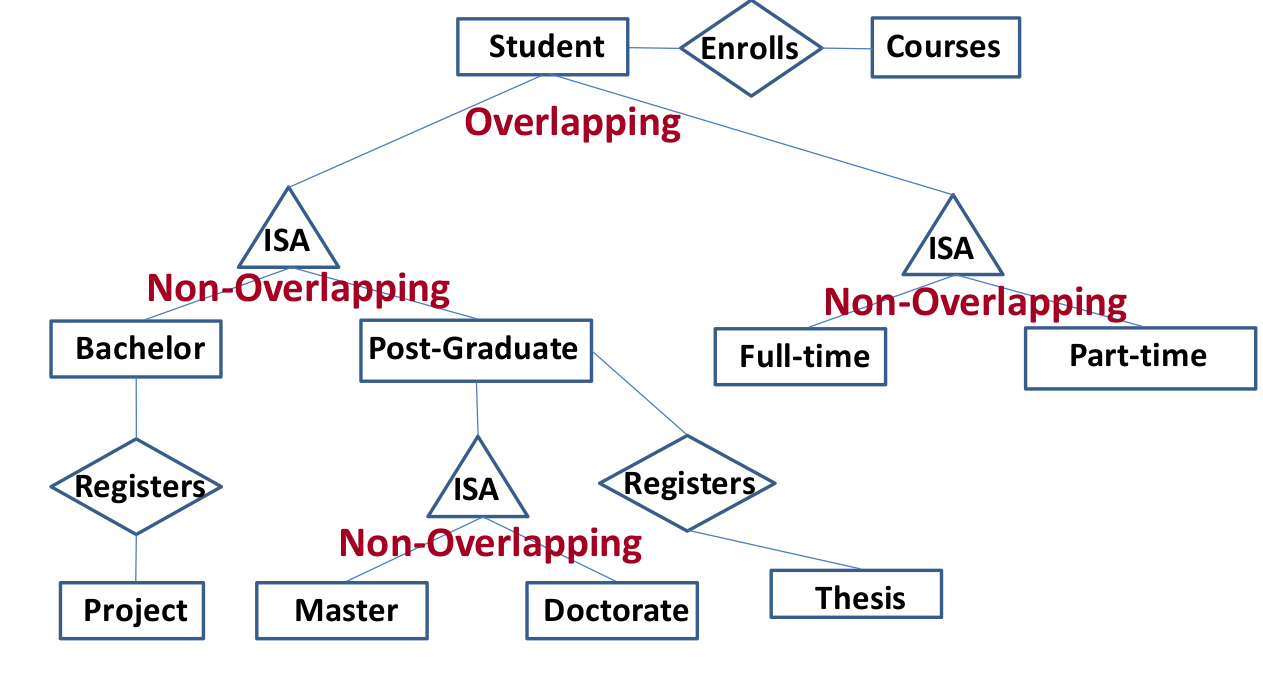
\includegraphics[width=.9\linewidth]{/home/raph/org/school/2016-2017/secondSemester/files/database_isa.png}
\end{center}
\subsubsection{Aggregation}
\label{sec:org4795cf9}
\begin{itemize}
\item Used to model a relationship involving a relationship set
\item Allows us to treat a relationship set as an entity set for purposes of
participation in (other) relationships
\end{itemize}
\subsection{Conceptual Design}
\label{sec:orgfdb282a}
\section{Lecture 3}
\label{sec:orga6241d7}
\subsection{Role of database system}
\label{sec:org4fe8c9b}
\begin{itemize}
\item Database: integrated, shared data collection
\item Integrated
\begin{itemize}
\item Eliminate needless redundancy
\end{itemize}
\item Maintain strong consistency
\item Shared
\begin{itemize}
\item Application written by programmers in multiple languages
\item End-users who use applications, forms, CLI to interact
\end{itemize}
\item Database systems shield users from
\begin{itemize}
\item How data is stored (bits \& bytes, 1 vs N files, 1 vs N disks\ldots{})
\item How data is accessed (btree, hashtable, scan, \ldots{})
\end{itemize}
\end{itemize}
\subsection{What is a data model?}
\label{sec:org0607429}
\begin{itemize}
\item Collection of application-visible constructs
\begin{itemize}
\item Describe data in application \& storage agnostic way
\end{itemize}
\item Constructs to describe structural aspects
\begin{itemize}
\item How do applications perceive the data?
\item Ex: table, graph, associative array\ldots{}
\end{itemize}
\item Constructs to describe manipulation aspects
\begin{itemize}
\item What operators can applications use?
\item Ex: join, traverse, lookup\ldots{}
\end{itemize}
\item Constructs to describe data integrity aspects
\begin{itemize}
\item How do we ensure that data manipulation is “correct”?
\end{itemize}
\end{itemize}
\begin{center}
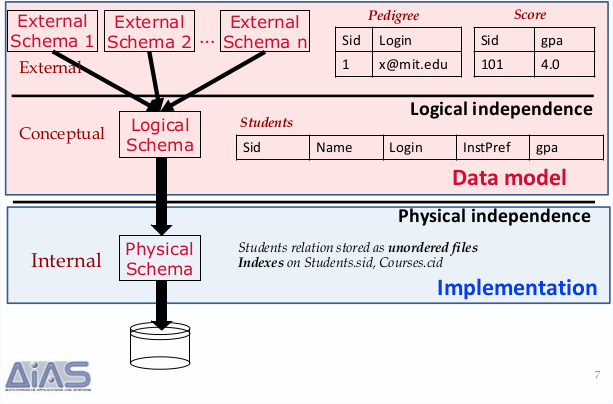
\includegraphics[width=.9\linewidth]{../../org/school/2016-2017/secondSemester/files/Lecture 3/screenshot_2017-03-06_10-36-55.png}
\end{center}
\subsection{Relation Model: Structural aspect}
\label{sec:org2eb9d44}
\begin{itemize}
\item Database = set of named \textbf{relations} (or \textbf{tables})
\item Each relation has a set of named \textbf{attributes} (or \textbf{columns})
\item Each \textbf{tuple} (or \textbf{row}) has a value for each attribute
\item Each attribute has a \textbf{type} (or \textbf{domain})
\begin{itemize}
\item integer, real, string, file formats (jpeg,\ldots{}), enumerated and many more
\end{itemize}
\item \textbf{Relation Schema}: relation name + field names + field domains
\begin{itemize}
\item Students(sid: string, name: string, login: string, age: integer, gpa: real)
\end{itemize}
\item \textbf{Relation Instance}: contents at a given point in time
\begin{itemize}
\item set of rows or tuples. (all rows are distinct with no specific ordering)
\item Cardinality: \# rows, Arity or degree: \# attributes
\end{itemize}
\item \textbf{Database Schema}: collection of relation schemas
\item \textbf{Database Instance}: collection of relation instances
\end{itemize}
\subsection{Relational Model: Integrity Aspect}
\label{sec:org291605e}
\begin{itemize}
\item Relational model provides \textbf{Integrity Constraints}
\begin{itemize}
\item condition specified on schema that restricts the data that can be stored in any instance
\item ICs are specified when schema is defined.
\item ICs are checked when relations are modified.
\end{itemize}
\item A \textbf{legal} instance of a relation is one that satisfies all specified ICs
\begin{itemize}
\item DBMS should not allow illegal instances.
\end{itemize}
\item With ICs, stored data is more faithful to real-world meaning
\begin{itemize}
\item Avoids data entry errors, too!
\end{itemize}
\end{itemize}
\subsection{Domain Constraints}
\label{sec:org231ec5c}
\begin{itemize}
\item Domain constraints: type of Integrity Constraints
\begin{itemize}
\item Domain specified in schema restricts the data that can be stored in that field
\end{itemize}
\item Enforced by the DBMS whenever tuples are added or modified.
\begin{itemize}
\item Similar to type checks in programming languages
\end{itemize}
\end{itemize}
\subsection{Relational Model: Keys}
\label{sec:org81e435b}
\begin{itemize}
\item Attribute whose value is \textbf{unique} in each tuple
\item Or set of attributes whose combined values are unique
\item Keys specify \textbf{key constraint}
\begin{itemize}
\item Enforced when tuples are inserted/updated
\end{itemize}

\item Key
\begin{itemize}
\item Set of attributes which uniquely identify a tuple
\end{itemize}
\item Candidate Keys
\begin{itemize}
\item If there are multiple keys, each of them is referred to as a candidate key
\item UNIQUE(licence\#)
\end{itemize}
\item Primary Key
\begin{itemize}
\item One of the candidate keys is chosen (by DBA)
\item PRIMARY KEY(sid)
\end{itemize}
\item Superkey
\begin{itemize}
\item Superset that includes a key
\item no two distinct tuples can have same values in all key fields
\end{itemize}
\end{itemize}

Key must be assigned carefully \(\Rightarrow\) must be specific
\subsection{Relational Model: Foreign Keys}
\label{sec:org5d7ee7c}
\begin{itemize}
\item Set of fields in one relation that `refer’ to a tuple in another relation
(like a pointer)
\item Foreign keys specify Foreign Key Constraint
\begin{itemize}
\item FK must correspond to the primary key of the other relation
\end{itemize}
\item If all foreign key constraints are enforced, referential integrity is achieved
(i.e., no dangling references.)
\item FOREIGN KEY (sid) REFERENCES Students(sid)
\end{itemize}
\subsubsection{Enforcing Referential Integrity}
\label{sec:orgb539f9e}
\begin{itemize}
\item What if an Enrolled tuple with a non-existent student id is inserted? (Reject it!)
\item What if a Students tuple is deleted?
\begin{itemize}
\item Also delete all Enrolled tuples that refer to it?
\item Disallow deletion of a Students tuple that is referred to?
\item Set sid in Enrolled tuples that refer to it to a default sid?
\item Set sid in Enrolled tuples that refer to it to a special value null, denoting `unknown ’ or `inapplicable ’ .
\end{itemize}
\item Can specify action taken on violation in SQL
\end{itemize}
\subsection{Mapping ER with key constraints}
\label{sec:orgc1c2b62}
\begin{center}
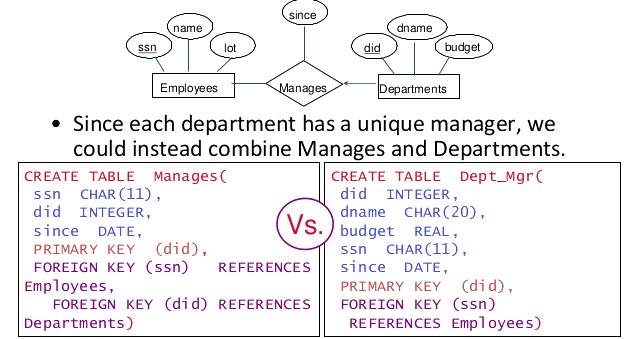
\includegraphics[width=.9\linewidth]{files/Lecture 3/screenshot_2017-03-06_11-36-30.png}
\end{center}
If no manager yet, could have a null ssn foreign key, maybe not what we want\ldots{}
\begin{itemize}
\item Does every department have a manager?
\begin{itemize}
\item If so, this is a participation constraint: the participation of Departments in Manages is said to be total.
\item Every did value in Departments relation must appear in a row of the Manages
relation (with a non-null ssn value!)
\end{itemize}
\end{itemize}
\begin{center}
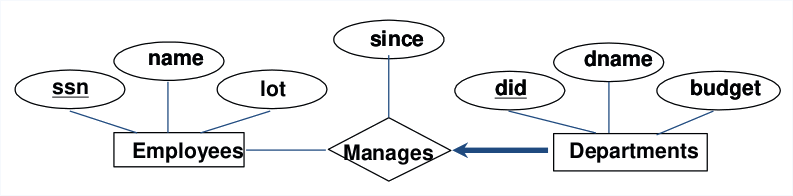
\includegraphics[width=.9\linewidth]{files/Lecture 3/screenshot_2017-03-06_11-50-07.png}
\end{center}
\begin{verbatim}
CREATE TABLE Dept_Mgr(
  did INTEGER,
  dname CHAR(20),
  budget REAL,
  ssn CHAR(11) NOT NULL,
  since DATE,
  PRIMARY KEY (did),
  FOREIGN KEY (ssn) REFERENCES Employees, ON DELETE NO ACTION)
\end{verbatim}
This way, department must have a manager
\subsubsection{Participation Constraints in SQL: Issues}
\label{sec:org235d8e2}
We cannot capture all participation constraints with PK, FK, not null
\begin{itemize}
\item Ex: Works\(_{\text{In}}\) relationship - total participation, no key constraint
\item Every did must must appear in a tuple in Works\(_{\text{in}}\) table
\item Cannot make did foreign key as did is not candidate key in Works\(_{\text{In}}\)
\end{itemize}
\begin{center}
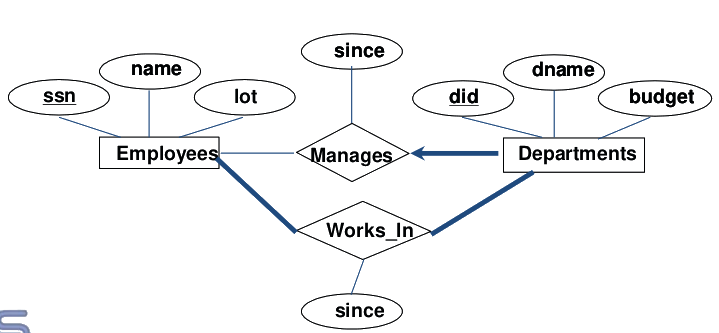
\includegraphics[width=.9\linewidth]{files/Lecture 3/screenshot_2017-03-06_11-45-33.png}
\end{center}
\subsection{Translating Weak Entity Sets}
\label{sec:orga85aa64}
Weak entity set and identifying relationship set are translated into a single table.
\begin{itemize}
\item When the owner entity is deleted, all owned weak entities must also be
deleted.
\end{itemize}
\begin{center}
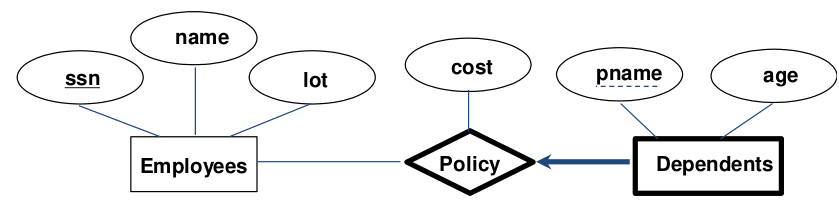
\includegraphics[width=.9\linewidth]{files/Lecture 3/screenshot_2017-03-06_11-51-38.png}
\end{center}
\begin{verbatim}
CREATE TABLE Dep_Policy (
  pname CHAR(20),
  age INTEGER,
  cost REAL,
  ssn CHAR(11) NOT NULL,
  PRIMARY KEY (pname, ssn),
  FOREIGN KEY (ssn) REFERENCES Employees, ON DELETE CASCADE)
\end{verbatim}
\subsection{Translating ISA Hierarchies to Relations}
\label{sec:org354a8a0}
\begin{center}
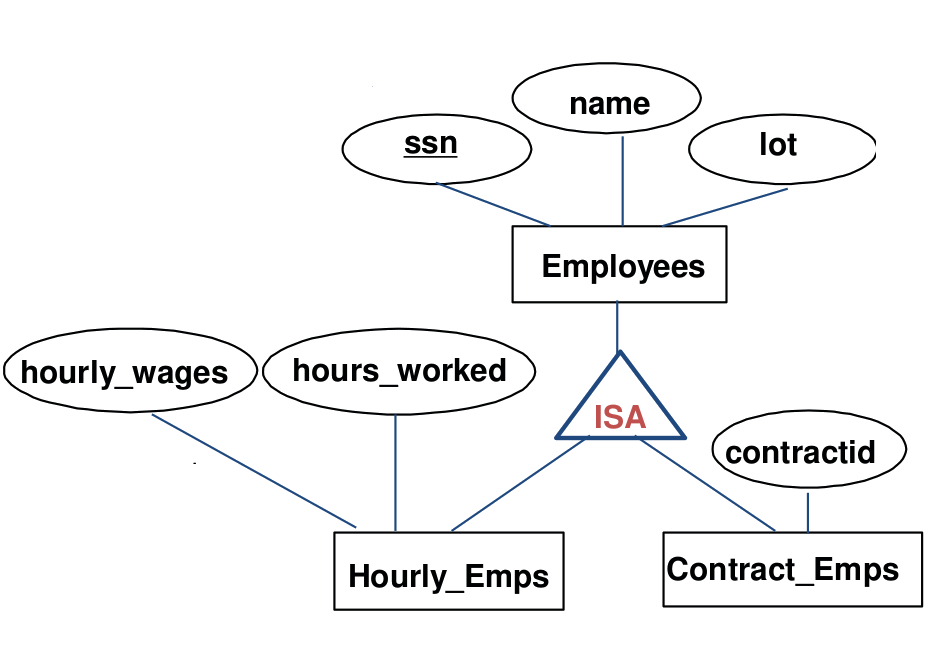
\includegraphics[width=.9\linewidth]{files/Lecture 3/screenshot_2017-03-06_11-54-01.png}
\end{center}
\subsubsection{Recall}
\label{sec:orgb8e2d72}
If we declare A ISA B, every A entity is also considered to be a B entity
\begin{itemize}
\item Overlap constraints: Can Joe be an Hourly\(_{\text{Emps}}\) as well as a Contract\(_{\text{Emps}}\)
entity? (Allowed/disallowed)
\item Covering constraints: Does every Employees entity also have to be an
Hourly\(_{\text{Emps}}\) or a Contract\(_{\text{Emps}}\) entity? (Yes/no)
\end{itemize}
\subsubsection{General approach}
\label{sec:org7969416}
3 relations: Employees, Hourly\(_{\text{Emps}}\) and Contract\(_{\text{Emps}}\).
\begin{itemize}
\item Every employee is recorded in Employees.
\item Hourly\(_{\text{Emps}}\): For hourly emps, extra info recorded in Hourly\(_{\text{Emps}}\)
(hourly\(_{\text{wages}}\), hours\(_{\text{worked}}\), ssn); must delete Hourly\(_{\text{Emps}}\) tuple if
referenced Employees tuple is deleted).
\item Queries involving all employees easy, those involving just Hourly\(_{\text{Emps}}\) require
a join to get some attributes.
\end{itemize}
\subsubsection{Alternative: Just Hourly\(_{\text{Emps,Contract}}\)\(_{\text{Emps}}\)}
\label{sec:org2c826b6}
\begin{itemize}
\item Hourly\(_{\text{Emps}}\): ssn, name, lot, hourly\(_{\text{wages}}\), hours\(_{\text{worked}}\).
\item Each employee must be in one of these two subclasses.
\end{itemize}
\subsection{NoSQL}
\label{sec:orgc1a3865}
\section{Lecture 4}
\label{sec:org79f8f96}
\subsection{Relational Query Languages}
\label{sec:org23c5707}
\begin{itemize}
\item Query languages: Allow manipulation and retrieval of data from a database.
\item Relational model supports simple, powerful QLs:
\begin{itemize}
\item Strong formal foundation based on logic.
\item Allows for much optimization.
\end{itemize}
\item Query Languages != Programming Languages!
\begin{itemize}
\item QLs not expected to be “Turing complete”.
\item QLs not intended to be used for complex calculations.
\item QLs support easy, efficient access to large data sets.
\end{itemize}
\end{itemize}
\subsection{Relational Algebra}
\label{sec:org9bdc6b6}
More operational, very useful for representing execution plans.
Since each operation returns a relation, operations can be composed! (Algebra is
5 basic operations.
\subsubsection{Selectiona and projection}
\label{sec:orgaac5dd6}
\paragraph{Selection (\(\sigma\) )}
\label{sec:org050bcc6}
Selects a subset of rows from relation (horizontal).
\begin{itemize}
\item Selects rows that satisfy selection condition.
\item Output schema of result is same as that of the input relation
\end{itemize}
E.g. \(\sigma_{\text{rating<9 \^{} age>50}}\)(S2)
\paragraph{Projection ( \(\pi\) )}
\label{sec:org91e4643}
Retains only wanted columns from relation (vertical).
\begin{itemize}
\item Retains only attributes that are in the projection list.
\item Output schema is exactly the fields in the projection list, with the same
\end{itemize}
names that they had in the input relation.
E.g. \(\pi_{\text{sname,rating}}\)(S2)
\begin{itemize}
\item Projection operator has to eliminate duplicates (How do they arise? Why remove them?)
\item Relational algebra is set based while SQL is bag (multiset) based
\end{itemize}
E.g. rows with same age, if project, should only get two ages, however in SQL,
we get them all\ldots{}
\subsubsection{Composing multiple operators}
\label{sec:org70d1d7f}
Output of one operator can become input to another operator.

E.g. \(\pi_{\text{sname,rating}}\)(\(\sigma_{\text{rating>8}}\)(S2))
\subsubsection{Union, Set Difference \& Intersection}
\label{sec:orgf9fd674}
\subsubsection{Cross-product ( X )}
\label{sec:org5d91e20}
Allows us to combine two relations.
\subsubsection{Set-difference (–)}
\label{sec:org46cb71e}
Tuples in r1, but not in r2.
\subsubsection{Union ( \(\cup\) )}
\label{sec:orge660747}
Tuples in r1 and/or in r2.
  “closed”).
\subsection{Relational Calculus}
\label{sec:org5307dad}
Lets users describe what they want, rather than how to compute it.
(Non-procedural, declarative.)
\end{document}